\chapter{PLUME laboratory testing}
\label{chap:labTests}

  The chapter~\ref{chap:vxd} has described the \gls{PLUME} project with the different prototypes that were built. 
  Since the version-1 of \gls{PLUME}, the detector is more complicated due to the six sensors on a module that have to be synchronised and the flex-cable which has a lot of thin metal traces to pilot and read the sensors.
  Before to perform test in real conditions at CERN or at DESY, the device has to be validated and characterised first in the lab.
  This chapter is introducing the different steps from the assembly procedure performed at Strasbourg (for the module) and Bristol (for a complete ladder), to the final tests with a radiation source, and include electrical functionality tests.

  %The \gls{PLUME} ladders are complex detectors and the last prototype was designed to optimise the material budget, by decreasing the width of the flex-cable and the metal traces.
  %Before to perform test in real conditions, the device has to be validated and characterised first in the lab.
  %This chapter is introducing the different steps from the assembly procedure performed at Strasbourg and Bristol, the electrical functionality checks to the tests with a radiation source,
 
 \minitoc
  
  %\begin{itemize}
  %  \item Describe bench
  %  \item Describe control of a sensor
  %  \item Describe output of Mi-26
  %\end{itemize}

\section{Visual inspection}

  The ladders are built in two steps. 
  Firstly, two independent modules are mounted at Strasbourg, then tested at DESY, to be then shipped at Bristol were the modules are glued together on a \gls{SiC}.
  The assembly procedure are introduced here and then the visual inspection is described.

  \subsection{Module and ladder assembly}

    \subsubsection{Module assembly}
    \label{subsec:modAssembly}

      The module assembly is performed at the IPHC by the microelectronics group and is done in three steps.
      First of all, the passive components are soldered onto a flex-cable.
      Then an epoxy layer with a thickness of $300 \mu\text{m}$ is glued under the connector side.
      This layer is used to reinforce the flex-cable on this non sensitive part due to the force applied by pulling and pushing the jumper cable.
      The module is then placed on a metal jig to insure its flatness thanks to a vacuum suction.
      The next step consists to glue the six sensors onto the flex.
      As they are thin and fragile pieces, the manipulation is done thanks to a vacuum sucker.
      Few drops of glue are dispensed on the flex and then the sensors are gently pressed one by one on top of it to be glued.
      The glue is then cured in a oven.
      The positioning of the sensors was used to be done manually, but a programmable robot is now in charge of it.
      The maximum mismatch alignment reaches $20 \mu\text{m}$. 
      The gluing procedure is definitive. 
      If a sensor is not working properly, it can't be removed and replaced by a new one because of the fragile flex-cable.
      On the worse case, a new sensor can be glued on top of it, but this procedure will increase the material budget.
      In order to avoid this situation, the sensors are probe tested at IK in Frankfort before the module assembly to select only the good ones.
      The final step consists to solder the 540 wire-bonds (a single MIMOSA-26 requires 90 wire-bonds) thanks to a semi-automatic machine.
      The wire-bonds can be protected by applying a glob top epoxy.
      It has the advantage to offer a protection against moisture ore contaminants, an electrically insulation and prohibits their movement during other manipulations. 
      Nevertheless, it increases the material budget on this area and if there is an electrical problem, the wire-bonds can't be disconnected.
      To test the module, it is transferred onto a plastic sole that has alignment pins.
      This sole is completed with a plastic cover to protect completely the module during shipping.

      %Control of absolute position about 10 $\mu\text{m}$.
      %Distance between edge of pixel of neighbouring sensors about $500 \mu\text{m}$.
      %Mismatch about $20 \mu\text{m}$.

      %The next step is to sold the wire-bonds (90 for a single Mi26) : semi-automatic machine
      %Modules are then transferred onto a plastic sole for testing and or shipping.

    \subsubsection{Ladder assembly}

    The ladder assembly is performed by the Bristol team.
    It consists to group two modules together on a spacer (\gls{SiC}) and a bate (an aluminum plate).
    The operation is done entirely by hands.
    Each module are placed on a separate jig thanks to alignment pins to ensure the positioning.
    The sensor side is facing the jig to have an access to the rear of the module for gluing.
    Then, the foam is placed on one module below the sensors, while the bate is glued below the connector with and overlaps the foam.
    The second module receives some glue on the backside before the jigs are assembled together.
    The glue is then cured for one day.
    The amount of glue needed for the assembly was studied carefully. 
    Indeed, the surface of the foam is not regular, so if not enough glue is used, the foam will not be glued on the module.
    On the other hand, using too much glue might stick the jigs together.
    When the ladder is finally ready, it is placed in an aluminum box used for shipping but also testing.
   
  \begin{figure}[!h]
    \centering
    \begin{subfigure}[t]{0.4\textwidth}
        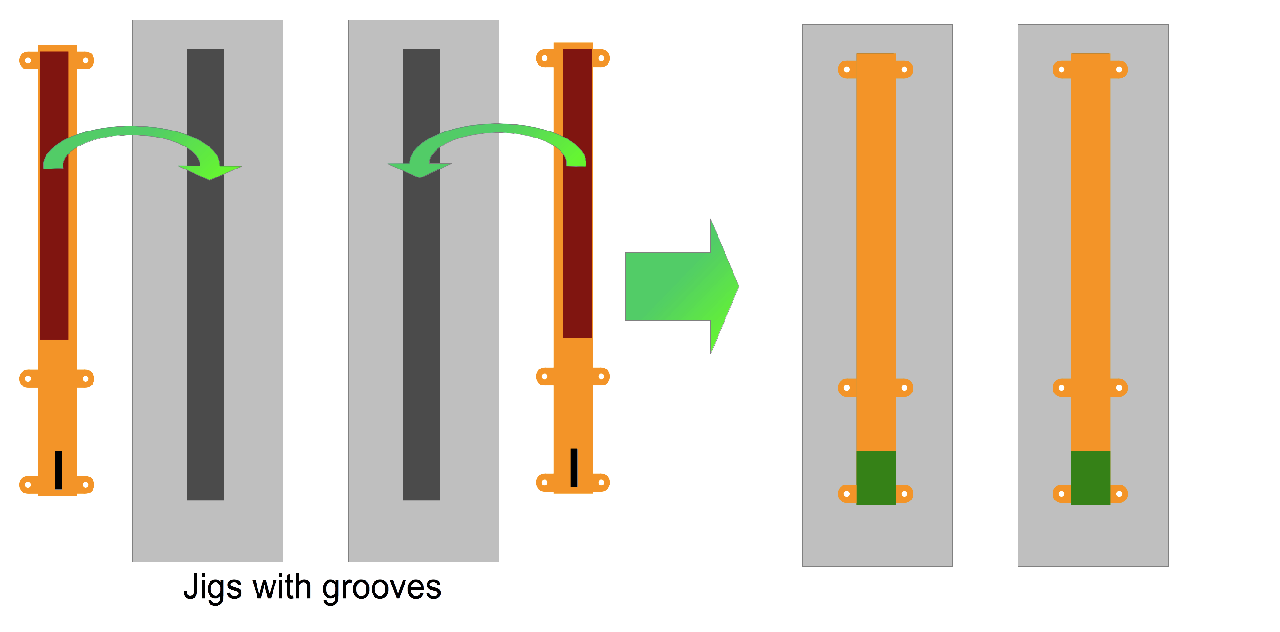
\includegraphics[width=1.3\textwidth]{Pictures/labTests/plumeLadderAssembly_step1.png}
        \caption{}
        \label{fig:ladderAssemblyStep1}
    \end{subfigure}
    \qquad
     %add desired spacing between images, e. g. ~, \quad, \qquad, \hfill etc. 
      %(or a blank line to force the subfigure onto a new line)
    \begin{subfigure}[t]{0.4\textwidth}
        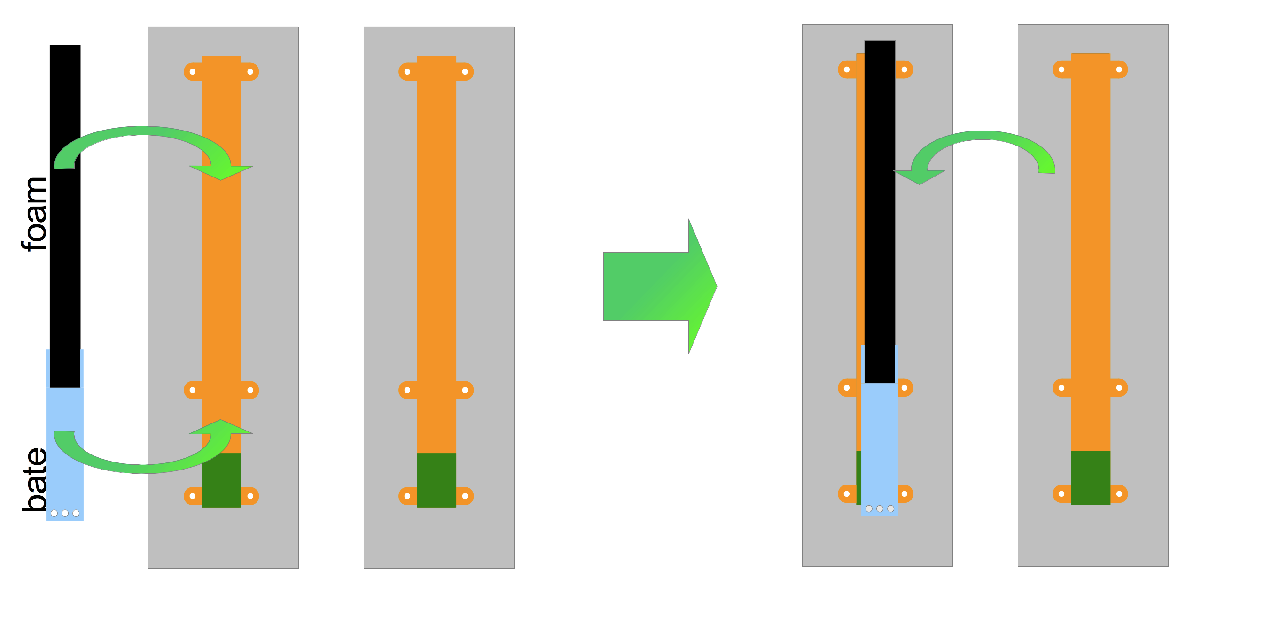
\includegraphics[width=1.3\textwidth]{Pictures/labTests/plumeLadderAssembly_step2.png}
        \caption{}
        \label{fig:ladderAssemblyStep2}
    \end{subfigure}
    \caption{Drawing of the ladder assembly. The modules are first placed on the jigs, sensors facing the grooves~\ref{fig:ladderAssemblyStep1}, then the foam and the bate are glued between the two modules~\ref{fig:ladderAssemblyStep2}.}\label{fig:ladderAssembly}
    \end{figure}    

  \subsection{Visual inspections}

  As explain in subsection~\ref{subsec:modAssembly}, the sensors positioning was performed firstly manually and later was switched to an automatic procedure.
  To tune properly the robot which is in charge of gluing the sensors on the flex-cable, the microelectronic group needs a position feedback.
  The modules are then inspected under a microscope to measure the gap between two sensors, and their position relatively to each other.
  The distance between the last pixel of a sensor to the neighboring one should be less than $500 \mu\text{m}$.
  The mismatch of the robot is about $20\mu\text{m}$. 
  The figure~\ref{fig:visAlign} is a picture taken with a microscope showing the relative position of two sensors on the bottom of the matrix for a aluminum straight module.
  %A visual inspection of the position,  as well as any problem on the matrix, as a crack, as well as a check of the wire-bonds have to be done before any electrical validation.
  The gap between the two edges is approximately $51 \mu\text{m}$. 
  
  \begin{figure}
    \centering
    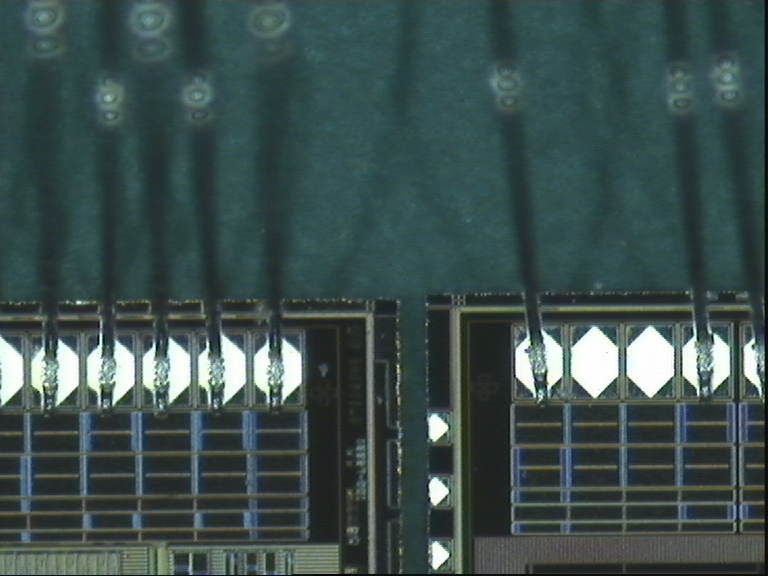
\includegraphics[width=0.6\textwidth]{Pictures/labTests/alignment_sensors.jpg}
    \caption{Visualisation of the alignment. The distance between the two edges is approximately $51 \mu\text{m}$.}
    \label{fig:visAlign}
  \end{figure}
  
  The visual inspection is also needed to check if the wire-bonds are correctly connected to the right sensor's pad, to verify that the gluing of the sensors on the flex-cable did not break the matrix and also to control that the shipping of the module between the labs (for example between Strasbourg and DESY) did not damage it.
  The module are fragile objects that have to be manipulated with care.
  Any wrong manipulation can damage severely the vital functionality.
  For example, the figure~\ref{fig:wireBondsCrashed} shows a picture taken with a microscope of wire-bonds crashed due to a falling cable on it.
  Because of the contact between some wires, the module was not working.
  Fortunately, the microcircuit group at Strasbourg was able to repair the damages and this module was operational then.
  To avoid this kind of accident to happen again, the modules were manipulated on a bench were the cables were tight and sheet of paper forbidden. 
  Therefore, the paper is able to chop off this wire.
  By using the glob-top method, the wire-bonded could have survived to a falling cable, but if the wire-bonds are not well assigned, there is no possibility to correct it.

  %\begin{itemize}
  %  \item Check positioning matrix defect (crack)
  %  \item Check wire bonds
  %  \item Check alignment
  %\end{itemize}

  \begin{figure}[!h]
    \centering
    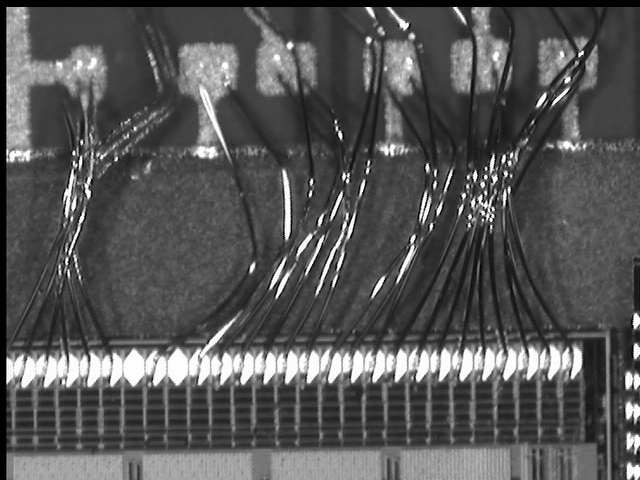
\includegraphics[width=0.6\textwidth]{Pictures/labTests/crash_bonds.jpg}
    \caption{Picture taken with a microscope showing wire-bonds crashed due to a falling cable.}
    \label{fig:wireBondsCrashed}
  \end{figure}

\section{Electrical validation}

  The electrical validation of a \gls{PLUME} module or ladder is performed in two steps.
  The first one consists to check that all the system controlling and powering the module is working. 
  Then, the module is connected and its consumption, as well as the communication are checked.

  \subsection{Auxiliary board}

  On one edge of the module, a ZIF connector is used to power the sensors, but also to pilot them and to transfer the data to the outside world.
  A jumper cable is connected between the module and an auxiliary board.
  This card is connected to a power supply board which is providing the nominal voltages needed by the module.
  The $\text{V}_{DD_d}$ and $\text{V}_{DD_a}$, used for the buffer, are tunable thanks to two potentiometers, while $\text{V}_{CC}$, used for buffers is fixed to 3.3 V.\todo{Look for VDD and VCC}
  The auxiliary board is also connected to a computer for the slow control.
  Two RJ45 are in charge to provide the JTAG registers, as well as the start, the reset signal and in a case of a complete ladder an external clock.

  First of all, the auxiliary board is connected to the power supply board which is plugged to two external power supplies, which are delivering  8 V D.C.
  The current of the empty auxiliary board should be about 350 mA.
  The first step is to check the different voltages on the auxiliary board.
  The $\text{V}_{CC}$, $\text{V}_{DD_d}$ and $\text{V}_{DD_a}$ should be at 3.3 V, but only the two last voltages can be adjusted thanks to potentiometers on the power supply board.
  The $\text{V}_{clp}$ is set to 2.1 V and should not be outside the range $\left[2, 2.2\right]$ V.
  An I2C chips or a potentiometer are providing this voltage.
  The auxiliary board has a section dedicated to the power pulsing, nevertheless, for the purpose of the electrical validation, the system is disconnected.

  The JTAG communication between the computer and the auxiliary board is then checked.
  One RJ45 connector is dedicated to the JTAG slow control. 
  Four signals are sent:
  \begin{description}
    \item[TDI (Test Data In):] received the serial data input feed to the test data registers or instruction register
    \item[TMS (Test Mode Select):] controls operation of test logic (for example, by selecting the register)
    \item[TCK (Test Clock):] uses to load test mode data from TMS pin and test data on TDI pin at the rising edge, while at the falling edge, it is used to output the test data on the TDO pin.
    \item[TDO (Test Data Out):] the output data feed the input data of the next sensor and the last sensor sends the information back to the computer 
  \end{description}

  The second RJ45 connector is providing signal coming from the DAQ:
  \begin{description}
    \item[Clock:] this line is used only to synchronise two modules together
    \item[Start:] The JTAG can't start multiple sensors. This signal is provided by the DAQ
    \item[Reset:] default value is 1 
  \end{description}

  The clock provided to the sensors should be at 80 MHz and is transmitted to the sensors via LVDS.
  The connections of the auxiliary board to the different component are summarised on figure~\ref{fig:plumeAux}.

  \begin{figure}[!h]
    \centering
    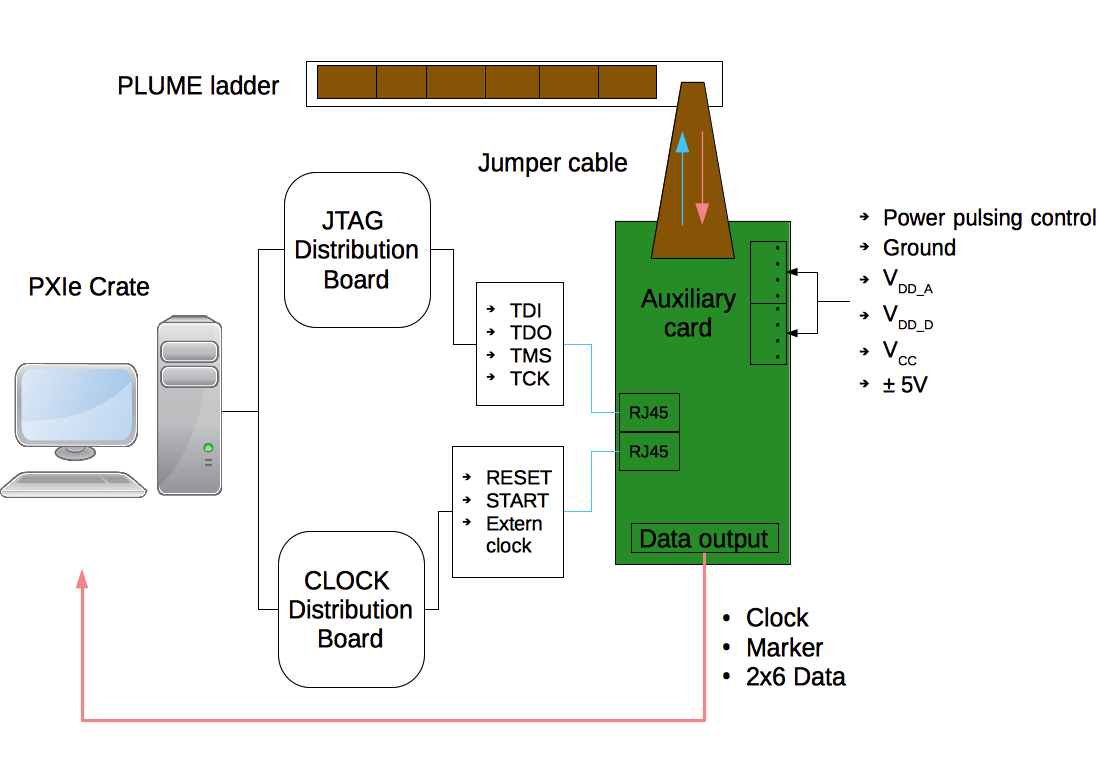
\includegraphics[width=\textwidth]{Pictures/labTests/plumeAux.png}
    \caption{Sketch of the PLUME connection.}
    \label{fig:plumeAux}
  \end{figure}


  %For the test procedure, but also for the acquisition, the PLUME module is connected to an acquisition board, via a jumper cable.
  %This board is in charge to distribute the power supplies, the control signals and the data output.
  %A power supply board is providing the $\text{V}_{dd_d}$ and $\text{V}_{dd_a}$, the $\text{V}_{CC}$ and 5 V.
  %The $\text{V}_{dd_d}$ and $\text{V}_{dd_a}$ are tunable thanks to two potentiometers, while $\text{V}_{CC}$ is fixed.

  %A PLUME module is connected to an auxiliary board via a jumper cable in order to be operated.
  %This auxiliary board is providing the power supply and the slow control to the ladder and give then an access to the sensors' output.
  %Two RJ45 inputs are providing the slow control, the reset and start signal and has the possibility to provide an external clock, used only when two modules are working together to make sure that they are synchronised.
  %A power supply board, connected to the auxiliary board, is providing the digital and analog voltage, plus 

  %An auxiliary board is in charge to power a PLUME module and to send the slow control to pilot each sensor. 
  %If only one module is tested, an oscillator is providing the 80 MHz clock.

  %Sixteen pads are used to read the response of the six sensors and the clock and marker of the sensor number 6.
  %It also has an output connection to check the response of each sensor with an oscilloscope, as well as for the acquisition.
  %It is in charge to provide the 80 MHz clock, via oscillator or via an external input. 

  %\begin{itemize}
  %  \item Generate the 80 MHz for the 6 Mi 26 by oscillator on board or by an external input.
  %  \item Bufferisation of the Digital signals sent to the chips (JTAG and control signals) and the digital signal provide by the 6 Mi26 to the DAQ in LVDS .
  %  \item Regulators for the power supply of the sensors.
  %  \item Power pulsing
  %  \item Current measurement
  %  \item test point for the DAC characterisation
  %\end{itemize}


  \subsection{Smoke test}

 %@ After the connections were controlled and before to connect the module to the bench, the different voltages has to be set.

  After switching-off every power supplies, the module is connected to the auxiliary board via a jumper cable.
  The power supplies are switched-on again.
  The module consumption is checked at every JTAG steps to make sure that there is no short-circuit.
  Just after powering-on everything, the six sensors of the module are starting in a random state and this information can't be used to observe any problem.
  After the reset of the registers, the total consumption should be around 33 mA.
  Then the registers are loaded and the consumption should be around 750 mA and read-back by the JTAG software.
  If at the reading step no error was discovered, the sensors can be operated and their consumption should be around 1300 mA.

  The next step is then to control the JTAG communication of every sensor.
  A JTAG file which is configuring the sensors in a normal mode (80 MHz with zero suppression output) is loaded.
  When the start signal is sent, all the sensors are synchronised, so the \textit{clock} and \textit{marker} is read only from one sensor.
  The output is checked in three steps, chip by chip thanks to an oscilloscope.
  First of all, the sensor is reset, the register are loaded and read back and then the start signal is sent. 
  Then the header and trailer are modified in the JTAG software and the registers are loaded again.
  The output should change with respect to the word loaded.
  Then, the response of the discriminators are checked, specifically to find pixels stuck in an opened position.

  \subsection{Mimosa-26 output}

  An inspection of the output with an oscilloscope is performed to check the slow control and to estimate the response of the sensor.
  The information provided by a sensor is contained in four output lines.
  On a PLUME ladder, all the sensors are synchronised, so only the clock and marker from the last sensor is provided.
  The clock is always present and its rate depends on the clock register. 
  In a normal mode, the rate is 80 MHz.
  The second output is the marker. 
  It is available in all modes and its signal last during 4 clock cycles (starting at the rising edge) and is used to know the beginning of the data transmission.
  The data itself are divided on two output \textit{Data0} and \textit{Data1}. 
  It contains the \textit{header} and \textit{trailer} that allows to detect the beginning and the end of a data transmission.
  The signal is composed of $2 \times 16$ bits and its configurable via the \gls{JTAG}.
  Then, 16 more bits are indicating the \textit{frame counter}.
  It corresponds to the number of frame since the chip was reset.
  After that, the \textit{data length} provides an information on the length of the useful data.
  The useful data \textit{state} and \textit{status}

  \begin{figure}[h]
    \centering
    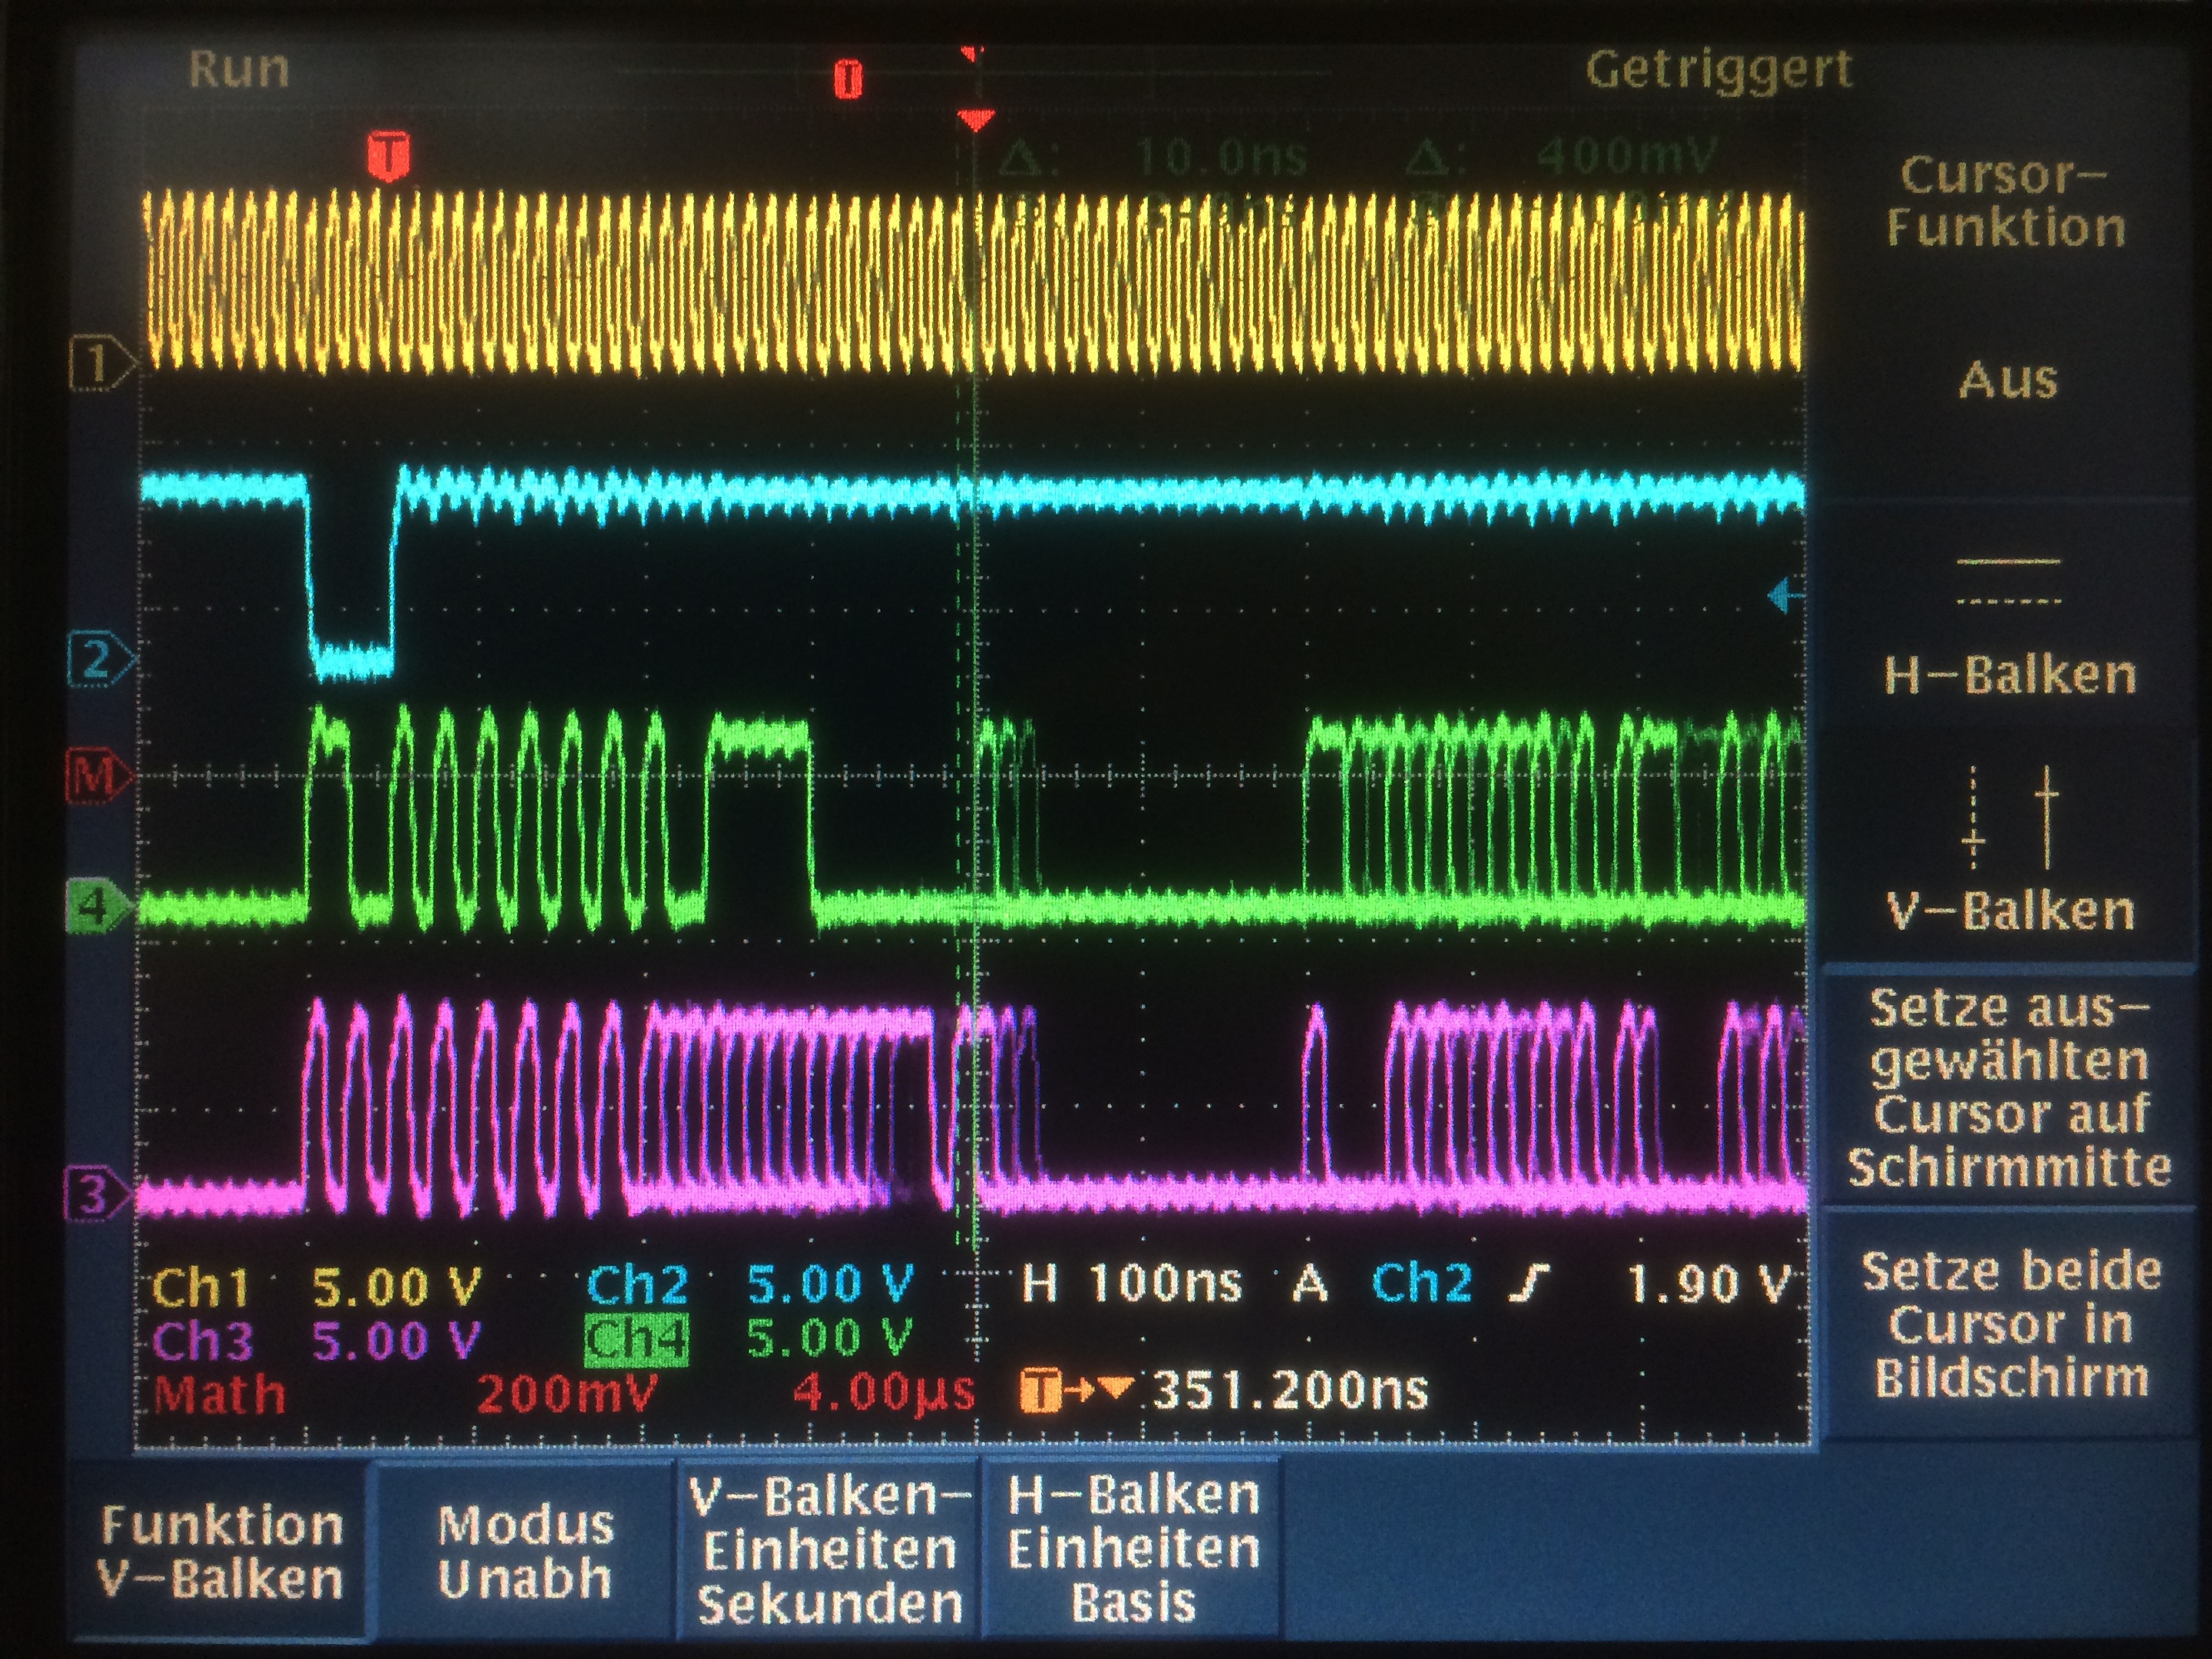
\includegraphics[width=0.8\textwidth]{Pictures/labTests/mi26_output}
    \caption{MIMOSA-26 output from oscilloscope. The top yellow line corresponds to the clock, the blue line below to the marker (which last 4 clock cycles), and the green and purple line are the data output containing the hit information}
    \label{fig:mi26Output}
  \end{figure}

\section{Noise measurements}

  In the chapter~\ref{chap:vxd}, the principle of the \gls{CMOS} sensors was described and the noise of this technology was discussed.
  The two noises contribution are the \acrfull{TN} and the \acrfull{FPN}.
  The measurement of the noise is needed to operate correctly the sensors, specifically to be able to detect physics signal. 

  \subsection{Threshold scan}

  The first step consists to configure the sensors for the discriminators output mode.
  The zero suppression mode is bypassed, pixels and discriminators are in normal mode (whole matrix read in $115\mu\text{s}$), but the readout frequency is lower (10 MHz) via 2 LVDS output pads.
  The control of the discriminators is divided into four sub-matrices, containing each 288 columns.
  The threshold voltage of this four blocks are defined in DAC unit in the JTAG software.
  A DAQ software is used to characterise each sensor. 
  By studying the baseline of a line in the middle of the matrix, the response of each matrix is set to a half activation by tuning the threshold of each sub-matrices.
  When the four thresholds are set, the homogeneity of the matrix is checked, as shown on the figure~\ref{fig:homogeneityMi26}.
  Then, the thresholds are set to the highest and lowest value to look for defect pixels.
  The figure~\ref{fig:openPixel} represents some pixels stuck in an open position.
  This mean that they are always activated and they will increase the fake hit rate of the sensor.
  If a part of a column is always opened, there is the possibility to disconnect the discriminator on the JTAG programm, otherwise, for a line, during an offline analysis, the line is not taken into account.
  The figure~\ref{fig:closePixel} represents some pixels stuck in a closed position.
  This pixels will never be activated and this area is not able to detect any particle.

  \begin{figure}[!h]
    %\centering
    \missingfigure{Homogeneity of the Mi26 matrix when the discriminators are 50 \% activated}
    \caption{Matrix response for the discriminators half activated.}
    \label{fig:homogeneityMi26}
  \end{figure}

  \begin{figure}[!h]
    %\centering
    \missingfigure{Output of closed pixels}
    \caption{Matrix response in discriminator mode, where all the discriminators are opened.}
    \label{fig:openPixel}
  \end{figure}
  
  \begin{figure}[!h]
    %\centering
    \missingfigure{Output of closed pixels}
    \caption{Matrix response in discriminator mode, where all the discriminators are closed.}
    \label{fig:closePixel}
  \end{figure}

  The second step consists to perform a threshold scan around the half activation point.
  At every thresholds, the response of each discriminators are recorded in order to calculate the noise, the offset and the dispersion.
  Usually, 29 runs with 500 to 1000 events are recorded.
  The scan can be done in two ways.
  The first one consists to inject a reference voltage in the discriminators while the matrix output is disconnected.
  In this way, only the noise contribution coming from the discriminators is measured.
  The second method does not use an external reference voltage, but rather the response of the pixel matrix to characterise the noise of the whole system.

  After completing the threshold scan, a configuration file, which contains the DAC values of each sub-matrix for each threshold with the corresponding value in millivolts is created.
  Then, the file is analysed and converted to create an output file containing a hit average picture of each sub-matrix for each step.
  Then a macro based on C++ and ROOT is reading this picture to plot the transfer function, as the one represented on figure~\ref{fig:transfer}, which shows the response of the 288 discriminators for a sub-matrix, as a function the threshold applied in millivolts.
  From this S-curve, the dispersion, as well as the offset and the noise are measured.
  Two plots are summarising this information, as shown on figure~\ref{fig:TN&FPN}.
  The one on the left represents the temporal noise, while the right one represents the fixed pattern noise.
  The offset corresponds to the RMS of the fixed pattern noise, the dispersion is the ... of ... and the noise ...
  To estimate the discriminator thresholds of each sub-matrix for a given \gls{SNR}, the total noise is determined as:
  
  \begin{equation}
    \text{Total noise} = \sqrt{<TN>^2 + <FPN>^2}
  \end{equation}

  For a given S/N cut $\sigma$, the thresholds are determined by:

  \begin{equation}
    \text{Threshold (mV)} = \text{Total Noise} \times \sigma + \text{offset}
  \end{equation}

  This is converted into the DAC values by taking into account the DAC offset and the DAC slope, which is assumed to be 0.25 mV:
  
  \begin{equation}
    \text{Threshold (DAC)} = \frac{\text{Threshold (mV)} - \text{DAC}_{offset}}{\text{DAC}_{slope}}
  \end{equation}
 
  \begin{figure}
    \centering
    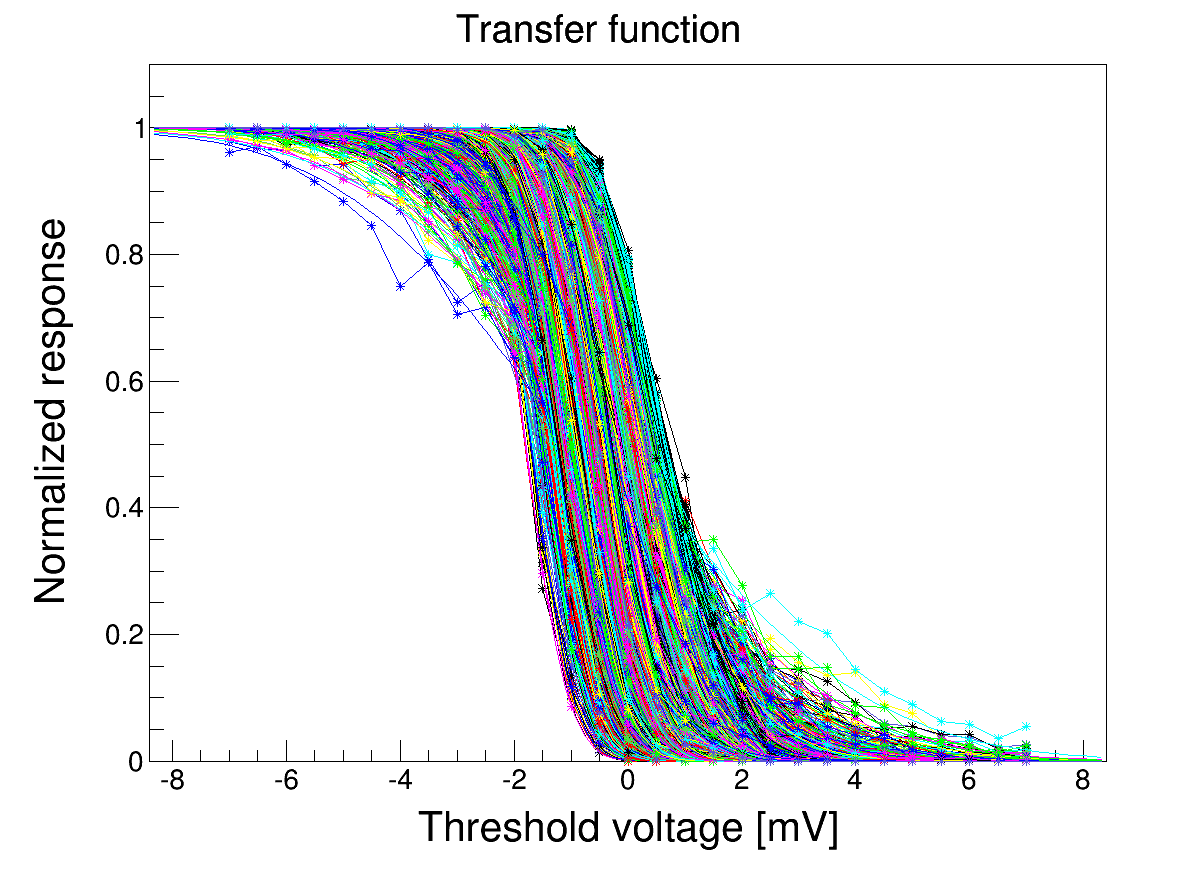
\includegraphics[width=0.6\textwidth]{Pictures/labTests/transfer_B.png}
    \caption{Pixels response of a threshold scan around the middle-point of discriminators for a sub-matrix.}
    \label{fig:transfer}
  \end{figure}

  \begin{figure}
    \centering
    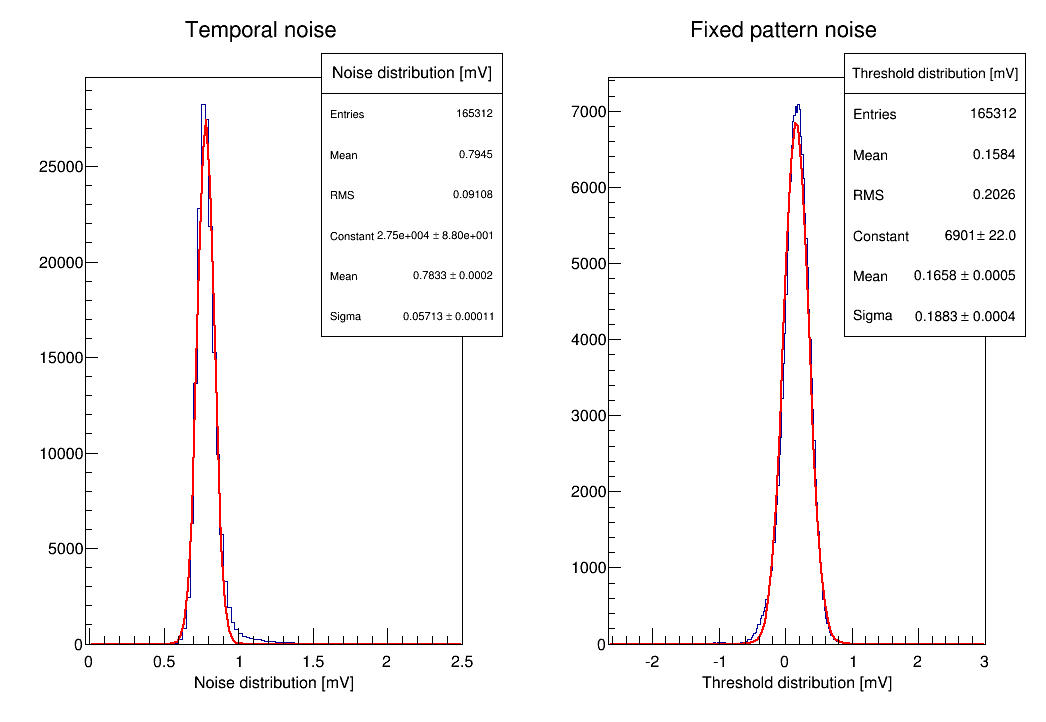
\includegraphics[width=0.8\textwidth]{Pictures/labTests/noise_A.png}
    \caption{TN and FPN}
    \label{fig:TN&FPN}
  \end{figure}

  Once the thresholds are defined for the different cuts, the fake hit rate of the matrix, as well as the detection homogeneity is determined.
  A quick step consists to use the DAQ software and acquire ten thousands event in a dark. 
  The fake hit rate per event per pixel is then determined as:

  \begin{equation}
    \text{F.H.R} = \frac{\text{Number of hits}}{\text{Number of events} \times \text{Number of pixels}} 
  \end{equation}
  
  The figure~\ref{fig:darkEvents} is representing the accumulation in the dark of ten thousands events for a threshold five times bigger than the noise.
  The measured fake hit rate was below $10^{-4}$ hits/pixel/events.

   \begin{figure}[!h]
    \centering
    
\includegraphics[width=0.6\textwidth]{Pictures/labTests/8sigma_10kEvents_noSource}
    \caption{Accumulation of 10k events at a thresholds of 5 times the noise acquired in the dark.}
    \label{fig:darkEvents}
  \end{figure}

  Then an iron 55 source is used to control the homogeneity of the thresholds determined before.
  The figure~\ref{fig:fe55} represents the accumulation of ten thousand events for a threshold five time bigger than the noise with a iron source on top of the sensor.
  
  \begin{figure}[!h]
    \centering
    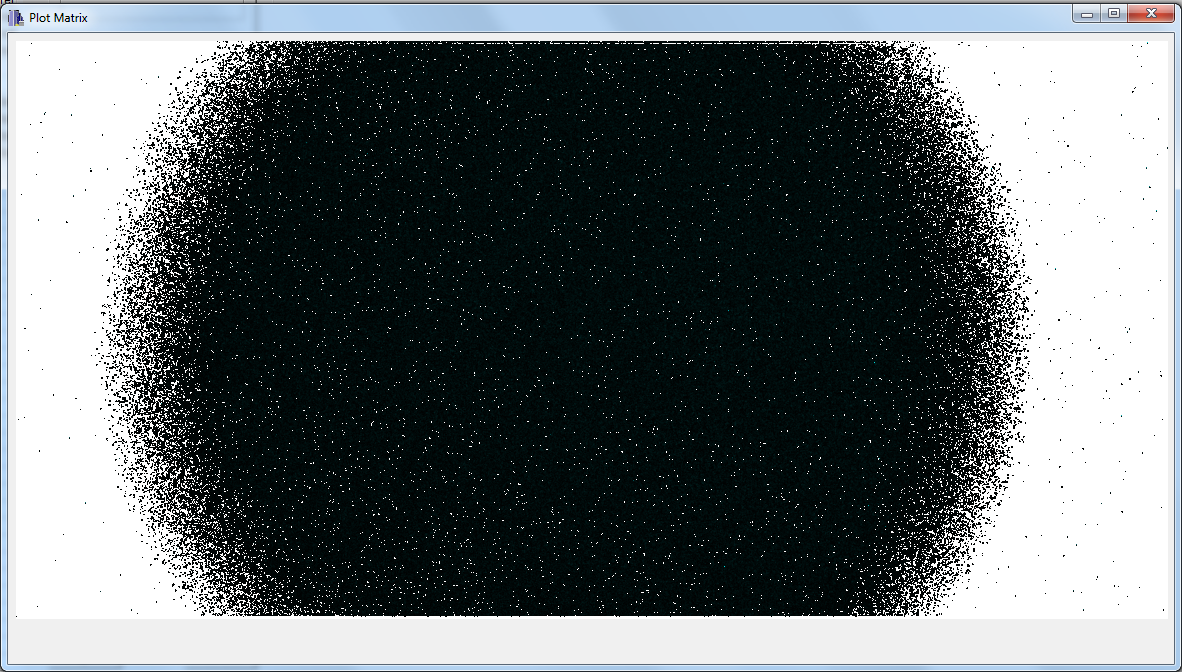
\includegraphics[width=0.6\textwidth]{Pictures/labTests/10kEvents_Fe55_cut5sigma.png}
    \caption{Accumulation of 10k events at a thresholds of 5 times the noise with Fe55 radiation source.}
    \label{fig:fe55}
  \end{figure}

  Finally, to validate the sensor, the acquisition system used during the test beam is used.\todo{detail the DAQ}
  Several runs containing each a million events are acquired for different threshold. 
  The data are stored in binary file that are read by a analysis program, called TAF and developed by the IPHC and based on C++ and ROOT.
  On the figure~\ref{fig:FHR}, the fake hit rate is represented. 
  The results are tallying the expectations for this sensors, as it was discussed on section .......

  \begin{figure}
    %\centering
    \missingfigure{FHR = f(Threshold)}
    \label{fig:FHR}
  \end{figure}

\section{Cluster}

  

  \begin{figure}
    %\centering
    \missingfigure{Cluster shape}
  \end{figure}
